\documentclass[11pt,twoside,english,singlespacing,headsepline,consistentlayout]{auxiliary/si-msc-thesis}

\usepackage[utf8]{inputenc} % Required for inputting international characters
\usepackage[T1]{fontenc} % Output font encoding for international characters

\usepackage{lipsum}
\usepackage{mathpazo}
\usepackage{setspace}

\usepackage{lipsum}
\usepackage{float}
\usepackage{listings}
\usepackage{wrapfig}
\usepackage{algorithm}
\usepackage{algpseudocode}
\usepackage{subcaption}
\usepackage{graphicx}
\usepackage{csquotes}
\usepackage{lscape}

\def\sectionautorefname{Section}
\def\subsectionautorefname{Subsection}

\usepackage{tikz}

\newcommand\encircle[1]{%
  \tikz[baseline=(X.base)] 
    \node (X) [draw, shape=circle, inner sep=0] {\strut #1};}

\lstdefinelanguage{algebra}
{morekeywords={import,sort,constructors,observers,transformers,axioms,if,
else,end},
sensitive=false,
morecomment=[l]{//s},
}

\newcommand{\quotes}[1]{``#1''}

\usepackage{listings}
\lstloadlanguages{Ruby}



%%%%%%%%%%%%%%%%%%%%%%%%%%%%%%%%%%%%%%%%%%%%%%%%%%%%%%%%%%%%%%%%%
%%%	MARGIN SETTINGS %%%%%%%%%%%%%%%%%%%%%%%%%%%%%%%%%%%%%%%%%%%%%
%%%%%%%%%%%%%%%%%%%%%%%%%%%%%%%%%%%%%%%%%%%%%%%%%%%%%%%%%%%%%%%%%

\geometry{paper=a4paper, inner=1.5cm, outer=1.5cm, bindingoffset=0cm, top=1.5cm, bottom=2.7cm, 
	%showframe, % Uncomment to show how the type block is set on the page
}

%%%%%%%%%%%%%%%%%%%%%%%%%%%%%%%%%%%%%%%%%%%%%%%%%%%%%%%%%%%%%%%%%
%%%	THESIS INFORMATION %%%%%%%%%%%%%%%%%%%%%%%%%%%%%%%%%%%%%%%%%%
%%%%%%%%%%%%%%%%%%%%%%%%%%%%%%%%%%%%%%%%%%%%%%%%%%%%%%%%%%%%%%%%%


\thesistitle{Sensorial software evolution comprehension}
\thesissubtitle{Summary} 



%comment to not have subtitle
% \thesissubtitle{Coarse-grained, Fine-grained, and Evolutionary\\ Software Visualization} 

\author{Gianlorenzo Occhipinti}

\monthyear{July 2022}

\supervisor{Prof. Dr. Michele Lanza}

% if you need to add or remove co-supervisors go into titlepage.tex and comment correspondingly

\cosupervisorone{Dr. Csaba Nagy}
\cosupervisortwo{Dr. Roberto Minelli}

%%%%%%%%%%%%%%%%%%%%%%%%%%%%%%%%%%%%%%%%%%%%%%%%%%%%%%%%%%%%%%%%%
%%%	FRONT MATTER %%%%%%%%%%%%%%%%%%%%%%%%%%%%%%%%%%%%%%%%%%%%%%%%
%%%%%%%%%%%%%%%%%%%%%%%%%%%%%%%%%%%%%%%%%%%%%%%%%%%%%%%%%%%%%%%%%

\begin{document}

\frontmatter
\pagestyle{plain}

%%%%%%%%%%%%%%%%%%%%%%%%%%%%%%%%%%%%%%%%%%%%%%%%%%%%%%%%%%%%%%%%%
%%%	CONTENT %%%%%%%%%%%%%%%%%%%%%%%%%%%%%%%%%%%%%%%%%%%%%%%%%%
%%%%%%%%%%%%%%%%%%%%%%%%%%%%%%%%%%%%%%%%%%%%%%%%%%%%%%%%%%%%%%%%%

%%%%%%%%%%%%%%%%%%%%%%%%%%%%%%%%%%%%%%%%%%%%%%%%%%%%%%%%%%%%%%%%%
%%%	TITLE PAGE %%%%%%%%%%%%%%%%%%%%%%%%%%%%%%%%%%%%%%%%%%%%%%%%%%
%%%%%%%%%%%%%%%%%%%%%%%%%%%%%%%%%%%%%%%%%%%%%%%%%%%%%%%%%%%%%%%%%

\begin{titlepage}

\hspace{-11.8mm} \includegraphics[width=65mm]{auxiliary/Grid-System-USI-Software.pdf}

\linespread{1.25}
\vspace{24mm} \hspace{26mm} \parbox{127mm}{{\bf {\huge {\textsc{\ttitle}}}\par}}
\linespread{1}

\ifthenelse{\boolean{@subtitle}}
	{\vspace{4mm} \hspace{26mm} \parbox{127mm}{{\bf {\large {\em {\subtitle}}}}}\vspace{10mm}}
	{\vspace{26.5mm}}

\vspace{16mm} \hspace{26mm} \parbox{127mm}{{\Large {\textbf{\authorname}}}}

\vspace{24mm} \hspace{26mm} {\large \moyear}

\vspace{48mm} \hfill {\large {\em Supervised by}}\\ \vspace{1mm} \hfill {\large {\bf {\supname}}}

\vspace{8mm} \hfill {\large {\em Co-Supervised by}}\\ \vspace{1mm} \hfill {\large {\bf {\cosupnameone}}}

%comment out if it does not apply

\vspace{1mm} \hfill {\large {\bf {\cosupnametwo}}}

%\vspace{1mm} \hfill {\large {\bf {\cosupnamethree}}}


\vfill

%\hfill \noindent {\textsc{Software \& Data Engineering Master Thesis}}

\end{titlepage}

\mainmatter
 
\pagestyle{thesis} 



\section*{Introduction}
Modern software systems are characterized by sheer size and complexity. As they grow, maintenance also takes a significant fraction of their life-cycle costs \cite{Davis1995, Sommerville1995, Erlikh2000, seacord2003}. The understanding activity to perform maintenance tasks (e.g., finding the causes of a bug) is a primary influencing factor of maintenance costs, among many others \cite{Corbi1989}.
Comprehending software evolution is essential for systems' understandability and, consequently, maintainability. However, the sheer quantity and complexity of the information generated during systems development challenge the comprehension process.

Numerous techniques have been presented in the literature to facilitate program comprehension \cite{Lanza2001, DAmbros2006, Steinbrueckner2010, Wettel2011, Alexandru2019, SoftwareEvolution}. The main challenge they have to deal with is identifying relevant aspects to be presented so that the user does not get lost in the myriad of information. Visualization techniques often support software evolution analysis.
The effectiveness of a software visualization technique could be enhanced by combining it with audio. The term \quotes{program auralization} was coined, for this reason, aiming to communicate information about the program in an auditory way.
Many researchers studied the advantages given by audio as a communication medium \cite{Alty1995, Vickers2004, Boccuzzo2009, McIntosh2014, Mancino2017}.

We present an approach based on synesthesia, the production of a sense impression relating to one sense by stimulation of another sense. The approach represents the evolutionary process through an interactive visual depiction of the evolving software artifacts complemented by an auditive portrayal of the evolution. Our technique models and mines large git repositories.
The approach is exemplified in SYN, a web application that enables sensorial software evolution comprehension.
We applied SYN to five real-life systems and presented interesting insights and reflections. SYN is developed as open-source software, and a live demo is publicly available.\footnote{\url{https://syn.si.usi.ch}}

\section*{Approach}
\begin{figure}[ht]
    \begin{center}
        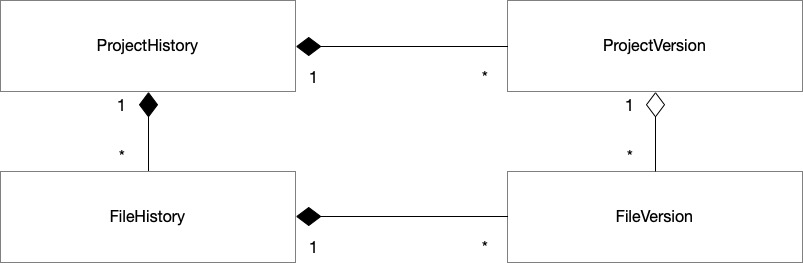
\includegraphics[width=0.6\textwidth]{images/approach/EvolutionModel.jpg}
    \end{center}
    \caption{Evolutionary Model}
    \label{fig:EvolutionaryModel}
\end{figure}


To model the evolution of software systems, we developed the model 
shown in \autoref{fig:EvolutionaryModel}. It is based on Hismo by Tudor Girba \cite{Girba2005}.
The need to develop a novel evolutionary model comes from the fact that Hismo was designed to work with another versioning system: Subversion (SVN). 
These are the four main concepts of our model: 
\begin{itemize}
    \item \textbf{ProjectHistory}: represents the history of a repository. It holds two sets: a set of FileHistories and ProjectVersions. 
    \item \textbf{FileHistory}: represents a repository file. We consider each file as an entity of the system. Even if the entity's name or location is changed, our mode will treat it as the same. So, our approach is resilient to renaming and moving activities. Each FileHistory holds a set of FileVersions, each representing a different entity version at a particular time.  
    \item \textbf{ProjectVersion}: represents a commit or a version of the system. 
    For each changed file in a commit, the respective ProjectVersion contains a FileVersion representing that change.
    A ProjectVersion holds contextual information about the commit, such as the timestamp, the hash of the commit, and its message.
    \item \textbf{FileVersion}: represents the version of a file at a particular point in time.
    It is responsible for holding all the evolutionary information of an entity. 
\end{itemize}

One of our goals was to analyze a large repository in an acceptable amount of time. 
In other words, our approach needs to be scalable. We present a scalable approach based on the concept of partial history.
A partial history holds information about a specific range of time of the ProjectHistory. 
It can be seen as a subset of a ProjectHistory. 
We can split the repository's history into multiple parts, each represented by a partial record. Then when their analyses are completed, we merge them to reconstruct the whole story of the repository.

Software systems are hard to understand due to the complexity and the sheer size of the data to be analyzed.
In our approach, we aim to make an interactive 3D representation to ease the comprehension task of a developer. 
To visualize a project, we introduce the concept of \textbf{view}. We define a view as a way to illustrate the evolution of a project given a set of specifications. This set of specifications determines how to build the view. For example, the colors and shapes of the entities, or the traversal of the evolution (e.g., by month or year) are configurable/part of the specification. A view holds a set of frames, called \textbf{AnimationFrame}, each representing the repository's state at a specific moment of its evolution. Therefore, the entire history of the repository is displayed by rendering AnimationFrames sequentially, like in a movie. 
We provide two visualization strategies to group commits into AnimationFrames: by timestamp and by commit. Both of them traverse the whole history from the beginning until the end.
To represent the system's state, an AnimationFrame holds a set of \textbf{ViewFigures}, each representing a system file and its visual properties such as its position, color, age, shape, opacity, and height.
Displaying abundant information on the screen might not be an efficient way to gather crucial aspects of the evolution of a software system. We want to play frames sequentially, like in a movie. Therefore, users might not have the time to understand the differences between the current and the previously displayed AnimationFrame. To overcome this issue, we provide an auditorial representation of an AnimationFrame to support understanding its changes. The goal is to support the sight sense, combining it with hearing, by playing audio notes that are recognizable by the user. Notes are generated from similar but complementary information of an AnimationFrame and help to understand it better. 

Generated sound melodies depend on the value of a pre-selected metric. For example, we can create a new metric to play how many Java files were added. In our approach, we assign distinct sounds to each metric, e.g., the number of commits will influence the tempo of our melody (i.e., beats per minute, BPM) and will be represented by a sound similar to a heartbeat.

The output of this approach is a piece of music representing a system's evolution. It is composed of a different sound/instrument for each metric. The idea is to use these values to control BPM, pitch, and the amplitude of a note. 

Therefore we designed and implemented SYN, a tool that supports the software evolution comprehension approach. 
It is composed of a set of modules, as follows:
\begin{itemize}
    \item \textbf{Core}: holds classes of basic SYN concepts such as ProjectHistory, ProjectVersion, and FileVersion. It also provides abstract classes, to define communication protocols and keep the implementation extensible.
    \item \textbf{CLI}: provides a Command Line Interface (CLI) to users.
    \item \textbf{Analyzer}: implements our scalable analysis. 
    \item \textbf{Server}: provides GraphQL endpoints to retrieve data. 
    \item \textbf{Visual Inspector}: used to debug and visually depict information collected during the analysis.
\end{itemize}  

\autoref{fig:SYNVisual} shows the Visual Inspector. Its interface is composed of four parts.
In box A, a 3D environment displays FileHistories on a virtual plane. The camera is not fixed, and the view angle and the zoom level can be controlled with the mouse. 
In box B, we have a card with general information about the project visualization. 
This card includes the project's name, the animation number, the dates of the animation frame, and its commit list. The slider shows the overall progress of the display, two buttons to jump to the subsequent or previous animation, and finally, one button to jump to the following animation with the time interval previously set. 
All the preferences specified during the project setup can be changed by clicking on the three dots in the top right corner.
In box C, we have a card to inform the user of the number of entities the UI renders. 
And finally, box D appears when an entity is selected with the mouse. 

The visual inspector is a helpful tool for understanding and debugging SYN's analysis process. However, it has performance issues in rendering large systems. The main problem stems from the browser environment as it has limited resources. We experienced a significant frame rate drop when rendering large systems. To overcome this limitation, we rendered large systems with POV-Ray,\footnote{\url{http://www.povray.org}} an open-source tool for creating high-quality three-dimensional graphics. We developed an extension of SYN that, given a View, produces a \texttt{pov} file for each AnimationFrame, following the same approach adopted in the visual inspector.  



\begin{figure}
    \center
    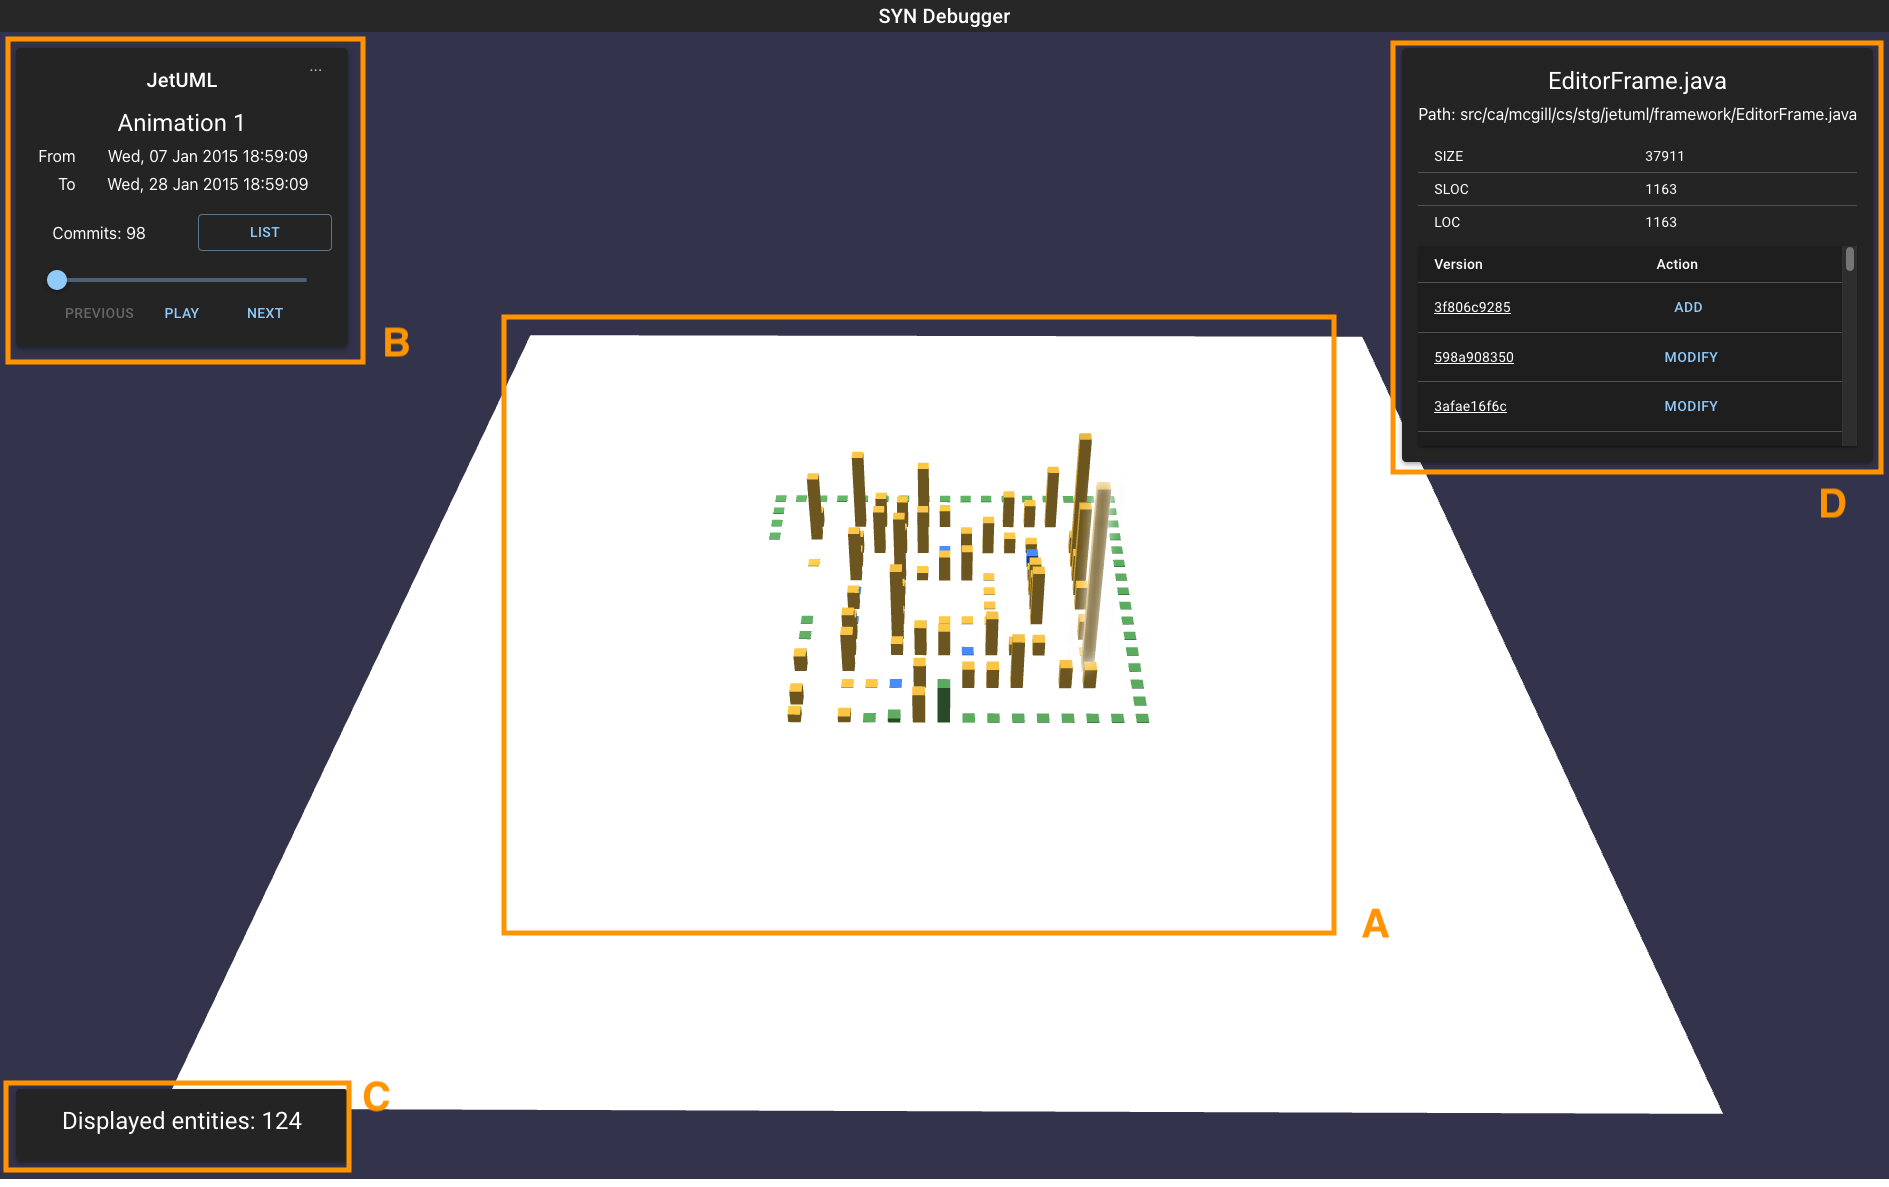
\includegraphics[width=\textwidth]{images/implementation/SYNUI-fileHistory.png}
    \caption{SYN Visual Inspector}
    \label{fig:SYNVisual}
\end{figure}

\section*{Case studies}
\graphicspath{ {images/casestudies} }





We applied SYN to real-life systems (shown in \autoref{tab:casestudies}) and presented several insights and reflections. 

\begin{table}[ht]
    \centering
    \begin{tabular}{lcrrr} 
        \hline
        {\bf Name} & {\bf First Analyzed Commit} & {\bf Last Analyzed Commit} & {\bf \# of commits} & {\bf \# of files}\\ 
        \hline
        JetUML & 07 Jan 2015 & 12 May 2022 & 2,152 & 795\\ 
        ArgoUML & 26 Jan 1998 & 29 May 2021 & 16,672 & 11,129 \\
        Elasticsearch & 28 Jun 2013 & 14 Apr 2022 & 34,842 & 41,043 \\
        LibreOffice & 07 Mar 2002 & 18 Jun 2022 & 367,996 & 213,791 \\
        Linux & 17 Apr 2005 & 19 Apr 2022 & 997,486 & 109,829
    \end{tabular}
    \caption{List of analyzed projects}
    \label{tab:casestudies}
\end{table}

The biggest project analyzed was Linux, with over 1 million commits. Its analysis took three days in 45 threads on a server with an AMD EPYC 7742 2.25GHz Processor. 

We combined our visualization and auralization approach in a video depicting the evolution of Linux.\footnote{\url{https://www.youtube.com/watch?v=iXGQoO7WAA0}}
The video shows how the Linux repository evolved in 17 years between April 2005 and April 2022. 

\autoref{fig:Linux_V7} shows a visual representation of sounds generated from Linux, with some frames of its evolution. The video starts with a peak on the number of files added. As we can see from AnimationFrame 1, the size of the system became massive in the first three months of evolution. Linus Torvalds, the author of Linux and the maintainer of the repository in April 2005, created a new repository to host the Linux codebase instead of converting the existing one to Git. He explained the reasons for this choice in the first commit. \footnote{\url{https://github.com/torvalds/linux/commit/1da177e4c3f41524e886b7f1b8a0c1fc7321cac2}}

In October 2008, as shown in AnimationFrame 14, there was a peak in the number of removed files. Consequently, the prevalence of the sound representing deleted files is high. In this video frame, the center of the spiral starts to become sparse. As highlighted in AnimationFrame 32, the development activity was constant and very high during this 
seventeen-year interval. This frame has many files painted with a bright color, meaning they were updated slightly before the frame's date. 
In the end, from AnimationFrame 68, we can understand the actual size of the system.

 We saw how the codebase of Linux evolved since their move to git. The development activity was constant throughout these 17 years. The codebase started with 19,705 files and reached 77,183 in April 2022, almost four times its original size. During this time, they evolved the kernel to develop new features and slowly started a process to remove the files that were added 17 years ago. As we can see, the center of the spiral began to become sparse. Nonetheless, it still holds many files, which means that the current version of Linux relies on files written more than 17 years ago. 

\begin{landscape}
    \Huge 
    \begin{figure}[ht]
    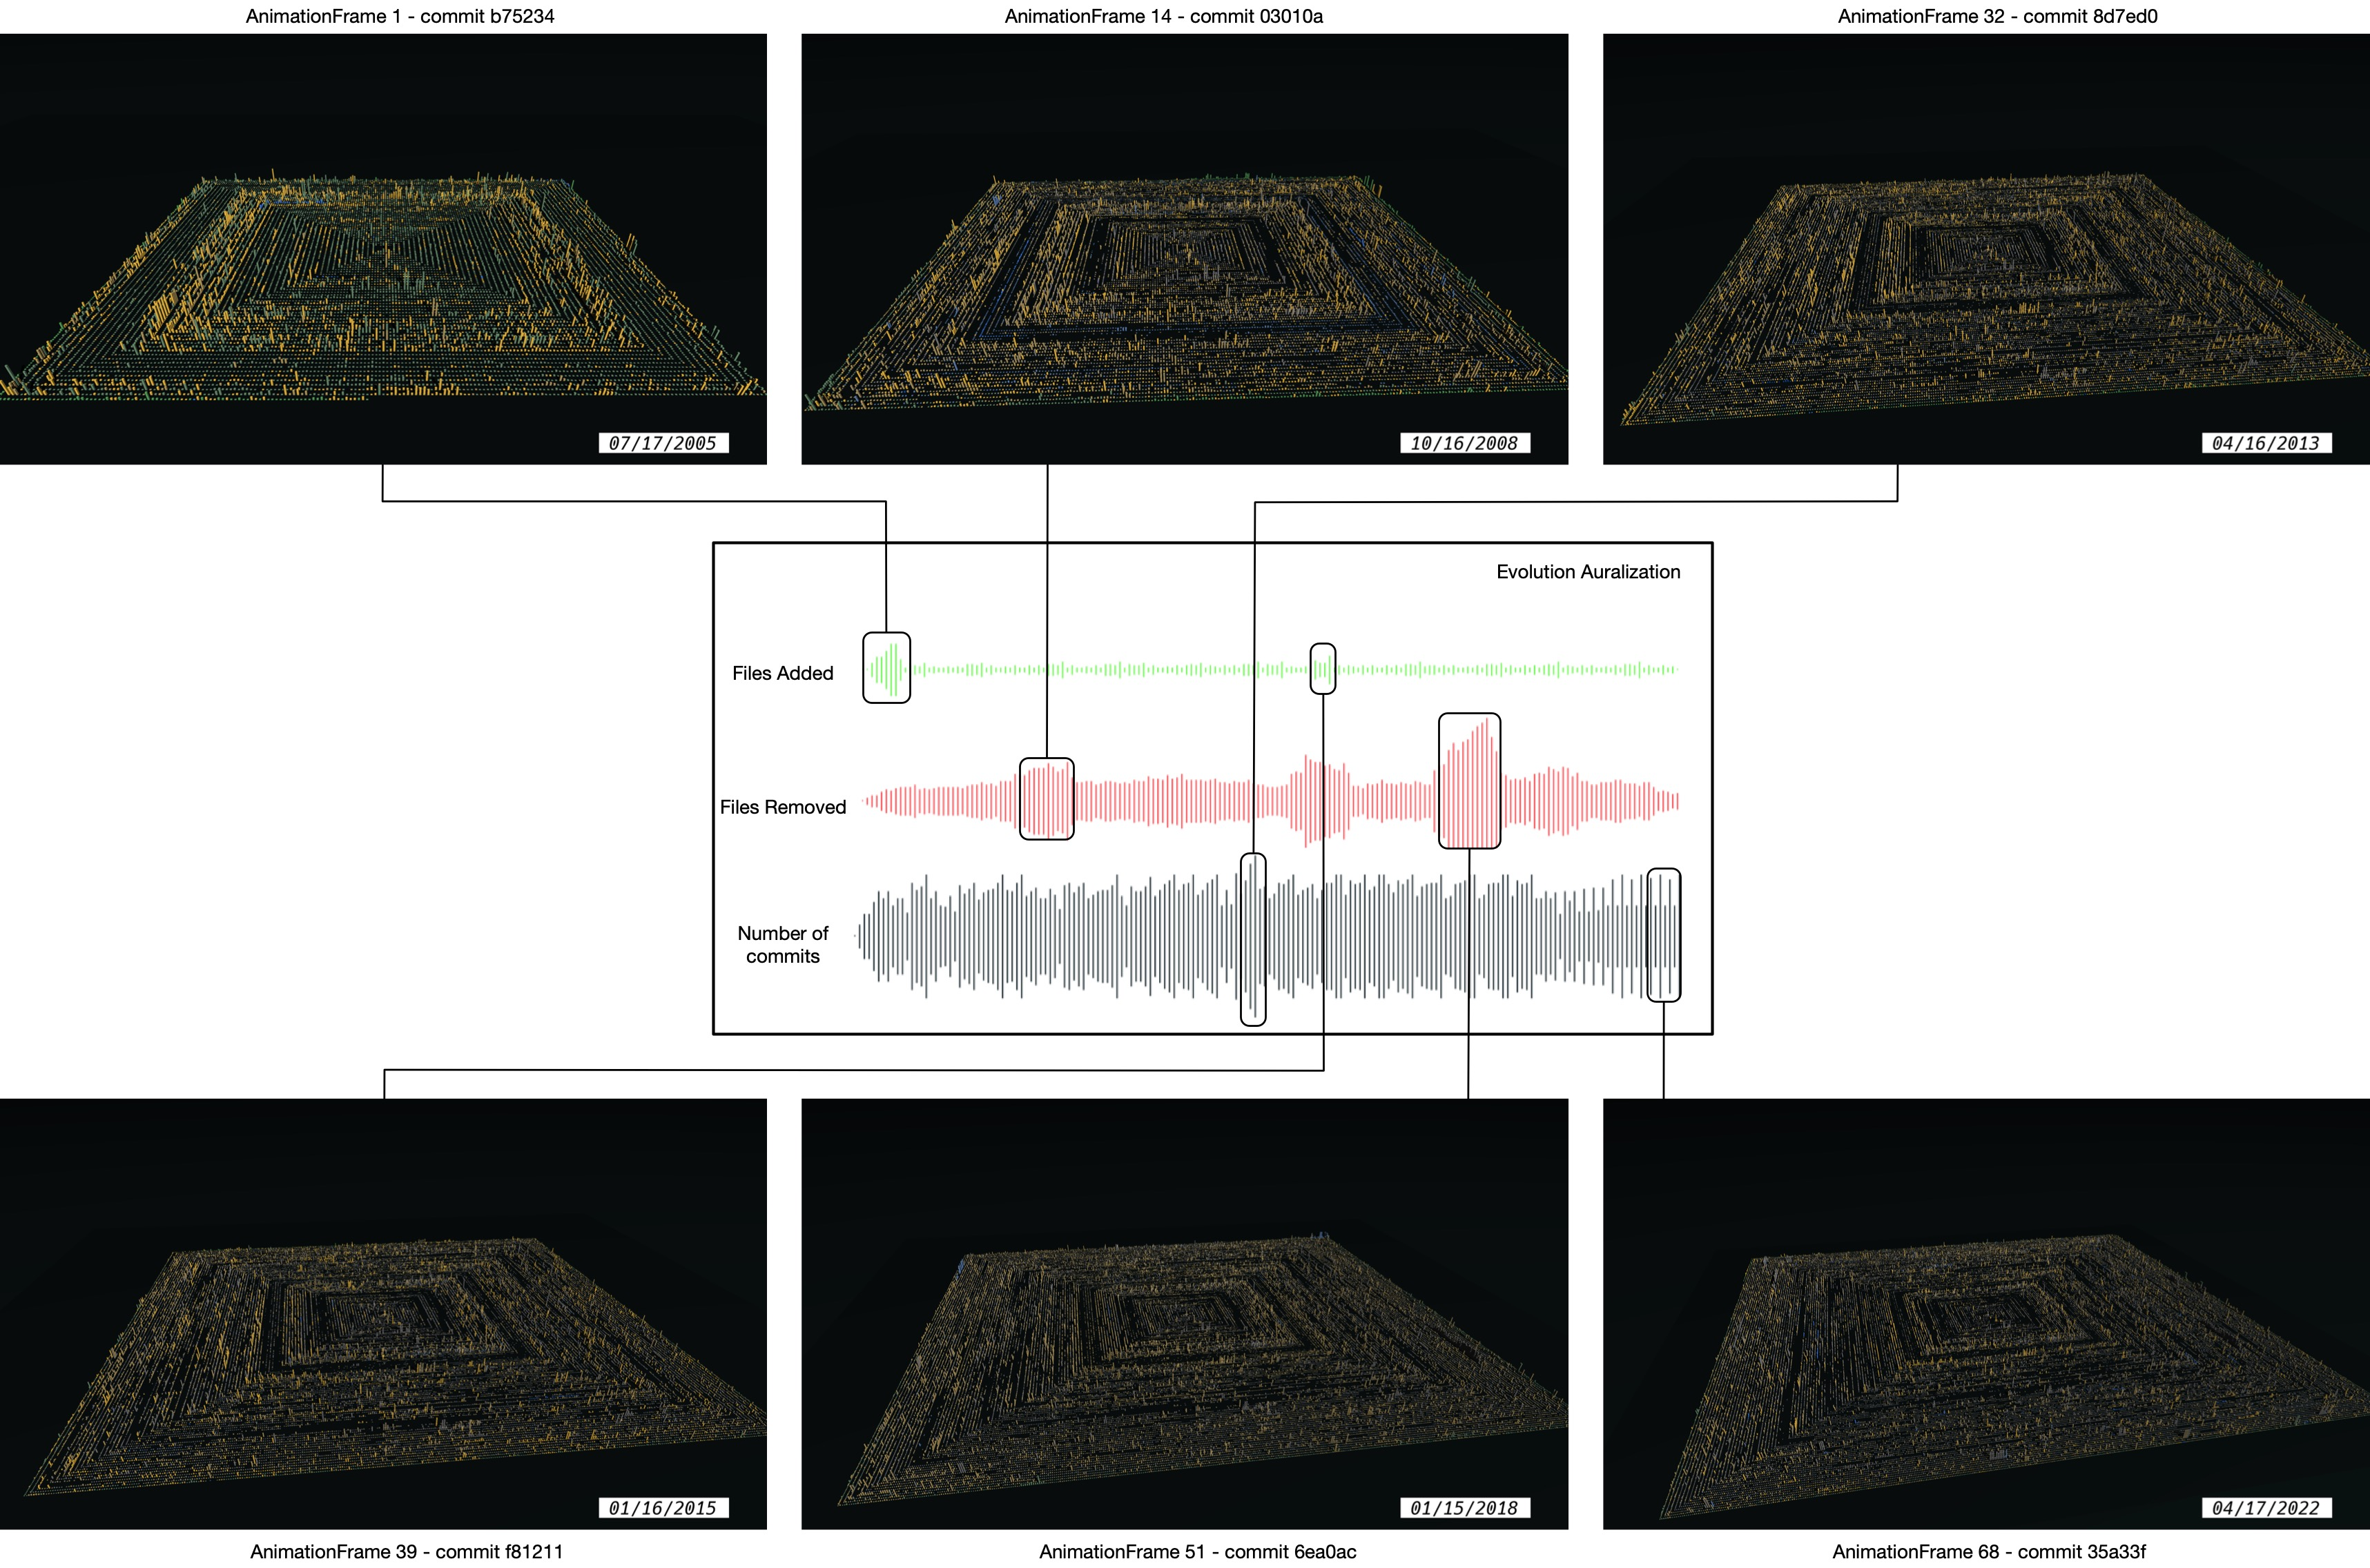
\includegraphics[width=\linewidth]{LinuxAuralization.jpg}
    \caption{Frames of Linux's Evoltution} 
    \label{fig:Linux_V7}
\end{figure}

\end{landscape}

\section*{Conclusions}

In the thesis, we presented an approach to mine, visualize and auralize large software repositories. The goal of this thesis was to explore new solutions to represent evolution. We cover all the stages required to reconstruct the history of a git repository, from the historical collection of information to the graphical data representation and visualization. We developed it with an agnostic approach against the programming language. Therefore, an extension of the system is needed to collect and visualize specific kinds of information. Our contributions can be summarized as follows:
\begin{enumerate}
    \item \textbf{The mining and modeling of a large git repository's history}. We present an approach to rebuilding the history of a git repository by traversing the repository's history. It starts from the first commit and analyzes all the subsequent commits until the end.
    We extract information about the modified files for each commit, parse it, and finally serialize it in a file on the local storage. The root element of our model is the history of a project that holds a set of files. An action recorded by a commit made on a file is also represented.
    \item \textbf{The sensorial software evolution visualization}. It exploits synesthesia, the production of a sense impression relating to one sense by stimulating another. It represents the evolutionary process through an interactive visual depiction of evolving software artifacts. It enables the comprehension of both the structural and the evolutionary prospectives. Moreover, SYN, the tool that implemented this approach, allows the user to customize visualization properties deeply. This approach provides the following benefits:
    \item \textbf{Auditive portrayal of the evolution}. It consists of a guideline suggesting how to compose audio sounds representing the evolution of a project. The proposed methodology was tested with two systems and presented with the JetUML and Linux case study analysis. The main benefit provided by this approach is the support of the visualization. It provides additional information without displaying them. Consequently, the listener can infer additional aspects of the analysis.
\end{enumerate}  

Overall, SYN presents a novel approach to visualize the evolution of a software system based on synesthesia. As we could see in the evaluation, SYN was helpful to spot interesting moments in the evolution of real software systems. It was also able to deal with extremely large, well-known software repositories such as Linux and LibreOffice. SYN opens the doors for several future research directions. For example, additional information, such as the author of the commit, can be retrieved from Git and employed in the visualization, or a new position layout that also considers the system's architecture could be developed. 
%%%%%%%%%%%%%%%%%%%%%%%%%%%%%%%%%%%%%%%%%%%%%%%%%%%%%%%%%%%%%%%%%
%%%	BIBLIOGRAPHY %%%%%%%%%%%%%%%%%%%%%%%%%%%%%%%%%%%%%%%%%%%%%%%%
%%%%%%%%%%%%%%%%%%%%%%%%%%%%%%%%%%%%%%%%%%%%%%%%%%%%%%%%%%%%%%%%%

\newpage
\bibliographystyle{abbrv}
\bibliography{biblio}

\end{document}